\section{Heatmaps and Geostatistical Mapping}\label{geostatistics}

%http://systems.cs.colorado.edu/~caleb/dyspan2012.pdf

Heatmaps are a valuable method of representing geostatistical data. As colour values on a map of some kind, in this case geographical, it allows the data to be visualised quickly and clearly, identifying any interesting points and features.

When measuring air quality values are only generally generated at points where sensors can easily be placed. With this project we are limited to roads, and indeed where the data collection algorithms have deemed it necessary to collect data. In order to effectively map air pollution a method of calculating the missing values must be found.

Geostatistics is a specific type of statistics which focuses on spatial data. One of the main uses being the prediction of values from a sample set, this being known as \emph{spatial prediction} or \emph{spatial interpolation}~\cite{practicalguidestatisticalmapping}. Within geostatistical mapping there is the ability to use many different interpolation algorithms. Indeed, \emph{A Practical Guide to Geostatistical Mapping of Environmental Variables} by Tomislav Hengl provides a list of just some of the available algorithms: 

\emph{``Inverse Distance, Kriging, Minimum Curvature, Polynomial Regression, Triangulation, Nearest Neighbour, Shepard’s Method, Radial Basis Functions, Natural Neighbour, Moving Average, Local Polynomial, etc.''}

When using this technique we must choose between a mechanical model and a statistical model. A mechanical model is suitable for the cases where no information about the data is available (e.g. range, deviation, mean, etc.). Statistical models use probability theory to estimate the new values using a provided rule set and can therefore be more accurate. 

Different types of each model will be looked at and compared in order to select the most suitable candidate for this project. However, the selection is dependent on factors such as the dataset it's self. This may mean that an accurate selection of model cannot be made until the data collection phase is complete~\cite{mappingairpollutionusinggis}. 

\subsection{Heat maps}\label{heatmaps}


\subsubsection{Definition}\label{heatmapdefinition}

A heat map is a two dimensional graphical representation of a matrix using colours to correspond to different magnitudes of values. It is a thematic map of a matrix, although can also be applied to geographical maps. 

\begin{figure}[H]
        \begin{center}
                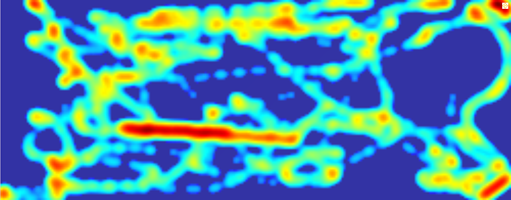
\includegraphics[scale=0.5]{./images/heatmaps/ExampleMouseMove.png}
                \caption{Example heat map generated from mouse movements}
                \label{fig:mousemoveheatmap}
        \end{center}
\end{figure}

Heat maps are generally used to quickly display which values in a matrix have the greatest magnitude and how they compare to surrounding values. Figure~\ref{fig:mousemoveheatmap}, which represents mouse movements on a website clearly shows a horizontal band in the middle which indicates that the users mouse spent a lot of time there. 

\paragraph{Calculations and Colour Progression} \hspace{0pt} \\


In order to create an image representation of the matrix, a colour progression must be chosen. The simplest colour progression method is a hue change on a single colour corresponding to the information. However this may not always be the most suitable method. When giving out information to the public, certain colours tend to represent different things. Red normally has negative connotations while green is the opposite. For this we can use a blended hue colour progression with red at one end of the scale and green at the other.


\paragraph{Representation Matrix} \hspace{0pt} \\

In order to generate the heat map we first need a matrix. A simple matrix can generate an effective heat map as can be seen from the following example.

\begin{figure}[H]
        \begin{center}
                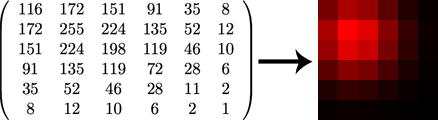
\includegraphics[scale=0.5]{./images/heatmaps/HeatMapGaussianExample.png}
                \caption{Heat Map Generation Example}
                \label{fig:matrixheatmapexample}
        \end{center}
\end{figure}

The example in figure~\ref{fig:matrixheatmapexample} has the maximum value of 255 represented by red (RGB value of \#FF0000) and the minimum value of 1 being almost black (RGB value \#010000). 

\emph{Missing Values}

With many applications there are either missing values in the matrix, or the values cannot be easily placed into a matrix (as is the case for geographical readings). To find the missing values, interpolation of some kind is used. In figure~\ref{fig:matrixheatmapexample} the matrix was generated by placing the value 255 in position (2,2) and performing a Gaussian blur with a filter size of 2 by 2 pixels and sigma equal to 2. 

Irregular data points must be processed further by mapping them onto a matrix. In the case of taking geographical readings, the heat map can be regenerated for each zoom level to ensure the maximum accuracy. 

These methods are not completely accurate and the missing data should be calculated in a manner appropriate to the application.

\subsubsection{Applications in Air Quality Measurement}\label{applicationsinaqmeasurement}

Heat maps are extremely useful to show the concentrations of pollutants in geographical areas. The information is easily given when overlaid on top of a map.  

\begin{figure}[H]
        \begin{center}
                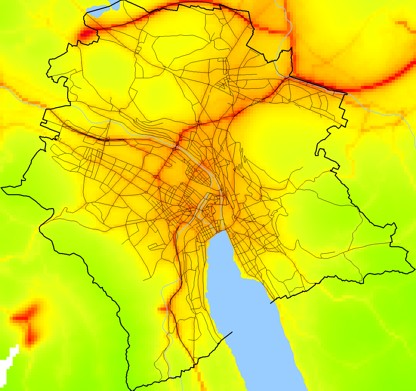
\includegraphics[scale=0.5]{./images/heatmaps/zurichpm.jpg}
                \caption{Particulate matter heat map in Zurich. Source: \url{www.stadt-zuerich.ch}}
                \label{fig:pmheatmapzurich}
        \end{center}
\end{figure}

From the above image we an easily see that the highest concentrations of particulate matter are where the roads are situated indicating a relationship between the two. 






\subsection{Mechanical Models}\label{mechanicalmodels}

\subsubsection{Inverse Distance Weighting}\label{inverseweight}
%http://www.alyrica.net/wifi_mapping

The key component of inverse distance weighting (IDW) is the calculation of new parameters as the weighted average of neighbouring parameters. The weight in this algorithm is calculated as the inverse of the distance from the current point to it's neighbours. The weighting is normalised so that the total of all weights to neighbours is equal to one. This causes the algorithm to slow down with large data sets and so a restriction on search radius may be put in place. 

\begin{figure}[H]
	\begin{center}
        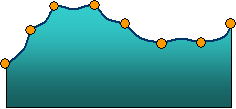
\includegraphics[scale=0.5]{./images/mpp1/IDW.png}
        \caption{Example of IDW. It is clear that it is not a ``perfect'' solution. Source: \url{http://esri.com}}
        \label{fig:idw}
	\end{center}
\end{figure}

\subsubsection{Regression on Coordinates}\label{regressiononcoordinates}

This model assumes that the value at any given point can be calculated using a function which also passes through, or goes close to, all other points. In this case of our three dimensional data (latitude, longitude and value) the function is the equation of a surface. Regression on coordinates does not use any information about the variance of the data. 

\subsection{Statistical Models}\label{statisticalmodels}

Many statistical models require no deliberate correlation between the measurements. Due to the fact that our measurements are taken along bus routes there is a definite correlation of geographic and temporal location information and therefore these models cannot be used. The main remaining model is kriging.

\subsubsection{Kriging}

Kriging is similar to IDW in that it follows the idea that an known point is the weighted average of it's neighbours. It is however more advanced in that it analyses the spatial structure of the data before any calculations take place~\cite{geostatisticalradiomapping}. It also takes into account environmental factors. This allows more accurate predictions. An example of how environmental factors are taken into account is when temperature is measured. IDW provides an answer based on nearby data. Kriging on the other hand would look at factors such as weather patterns, whether there are large bodies of water nearby, elevation, time of year, etc. All this data together allows kriging to be much more effective than simple IDW, however has the disadvantage that these environmental factors also need to be collected. There are 3 main types of kriging:

\begin{itemize}
	\item Ordinary kriging

		Ordinary kriging requires the construction of a variogram~\cite{ordinarykriging}. A variogram is a function which describes the degree of dependence of a spatial field as a function of distance and consists of two parts: an experimental variogram and a model variogram. The experimental variogram is calculated as the variance of each point in the data set plotted against the distance between the two. The model variogram is a simple mathematical function which models the trend of the experimental variogram. Examples of this can be seen in figure~\ref{fig:ordinarykrigingexample}.

		\begin{figure}[H]
        	\begin{center}
                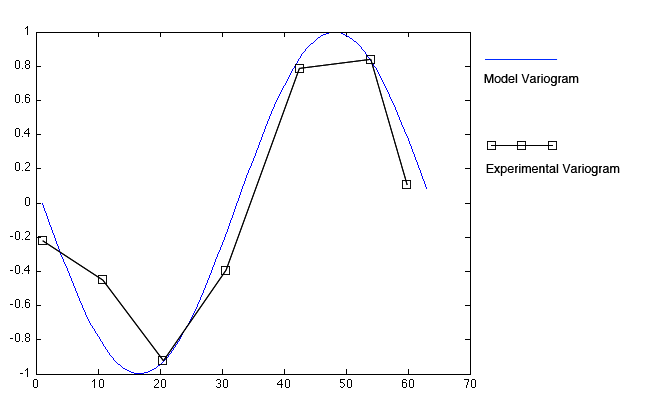
\includegraphics[scale=0.75]{./images/mpp1/KrigingModelFunction.png}
                \caption{Example experimental and model variograms}
                \label{fig:ordinarykrigingexample}
        	\end{center}
		\end{figure}

		When using kriging, as estimate of the variance is also returned with the interpolated results.

	\item Simple kriging

		Simple kriging is similar to ordinary kriging but it does not have the constraint that the weights surrounding a point must add up to one. This produces a less accurate but smoother result. ~\cite{simplekriging}

	\item Universal kriging

		Universal kriging assumes a stationary data set~\cite{universalkriging} and a polynomial trend model. The local trend implemented as part of this model provides some of the most accurate results

	\item Regression kriging

		Regression kriging is universal kriging but uses simple kriging to calculate the interpolated values of the environmental parameters provided to the algorithm ~\cite{regressionkriging}. 

\end{itemize}



\subsection{Comparison}\label{interpolationcomparison}

Each model has advantages and disadvantages. Both have lots of exposure to these types of environmental problems. 

In general the mechanical models are easier to implement, require less data and are faster. They have the downside that they are generally much more inaccurate. 

Statistical models are much more difficult to implement and take longer to run. They also require much more data about the environment in order to be as accurate as possible. This data varies and is dependent on what is being measured. In this case we would need information such as road layout, traffic density, building locations and heights, altitude, etc. Generally when being used in similar projects, the calculations are done by software such as \emph{ArcGIS}~\cite{arcgis}, which is unsuitable for this project due to the high cost of \$2500. Free alternatives exist for GIS software but only one of these has the ability to perform kriging. 

With the complexity in mind it would take longer than the project time frame to implement these statistical models. The extra information required would also provide extra difficulty, requiring either a third party data source or extra hardware. It would also be extremely difficult to validate the results. 

The choice is therefore to use a mechanical model. IDW is the simplest and is therefore the choice. While it is not as accurate as may be hoped in this application, the algorithm still provides a reasonable view of the data which is suitable for plotting on a map. A smoothing function may be required as IDW can cause patterns in the data as can be seen in figure~\ref{idw}.

Time permitting, the regression on coordinates model will be implemented and compared in order to find which is most suitable. 

\subsection{Alternative Methods}\label{interpolationalternatives}

\subsubsection{Compressive Sampling}\label{compressivesampling} 


The general principle behind compressive sampling is choosing the locations, both spatial and temporal, where measurements are taken in order to take the smallest number of measurements, whilst still allowing as much of the true data to be reconstructed as possible. The algorithm is similar to that used by JPEG compression. While this is a complicated technique, it would allow us to collect less data but still provide relevant results. However, this technique is more suited to taking measurements just along the roads rather than allowing us to interpolate missing data between roads. For this reason interpolation and extrapolation will be used, but this is an open area which may be revisited before the end of the project.




